%%%%%%%%%%%%%%%%%%%%%%%%%%%%%%%%%%%%%%%%%%%%%%%%%%%%%%%%%%%%%%%%%%%%%%%%%%%
% Definitions                                                             %
%%%%%%%%%%%%%%%%%%%%%%%%%%%%%%%%%%%%%%%%%%%%%%%%%%%%%%%%%%%%%%%%%%%%%%%%%%%
\gdef\version{1.0}
\gdef\doctype{Evaluation Sprint}

\documentclass[11pt]{article}
%Gummi|065|=)

\usepackage{eurosym}
\usepackage{listings}
\usepackage{color}
\usepackage[dvipsnames]{xcolor}
\usepackage{graphicx}
\graphicspath{ {.} }
\usepackage{upgreek}
\usepackage{titlesec}
\usepackage{fancyhdr}
\usepackage{tabulary}
\usepackage[utf8]{inputenc}
\usepackage{lastpage}


%for code snippets
\lstset{
  language=C,                	  % choose the language of the code
  %numbers=left,                   % where to put the line-numbers
  stepnumber=1,                   % the step between two line-numbers.
  numbersep=5pt,                  % how far the line-numbers are from the code
  backgroundcolor=\color{white},  % choose the background color. You must add \usepackage{color}
  showspaces=false,               % show spaces adding particular underscores
  showstringspaces=false,         % underline spaces within strings
  showtabs=false,                 % show tabs within strings adding particular underscores
  tabsize=2,                      % sets default tabsize to 2 spaces
  captionpos=b,                   % sets the caption-position to bottom
  breaklines=true,                % sets automatic line breaking
  breakatwhitespace=true,         % sets if automatic breaks should only happen at whitespace
  title=\lstname,                 % show the filename of files included with \
}


%%%%%%%%%%%%%%%%%%%%%%%%%%%%%%%%%%%%%%%%%%%%%%%%%%%%%%%%%%%%%%%%%%%%%%%%%%%
% Header                                                                  %
%%%%%%%%%%%%%%%%%%%%%%%%%%%%%%%%%%%%%%%%%%%%%%%%%%%%%%%%%%%%%%%%%%%%%%%%%%%
\renewcommand{\headrulewidth}{0.4pt}
\renewcommand{\footrulewidth}{0.4pt}
\renewcommand{\arraystretch}{1.4}
\fancyhead{}
\fancyfoot{}
\pagestyle{fancy}
\lhead{{\doctype}}
\rhead{{\fontfamily{phv}\selectfont \textcolor{gray}{Urban Green}} 
\includegraphics[height=0.8cm]{logo}}
\lfoot{Version \version}
\rfoot{\thepage\ von \pageref{LastPage}}
\setlength{\headheight}{30pt}


%%%%%%%%%%%%%%%%%%%%%%%%%%%%%%%%%%%%%%%%%%%%%%%%%%%%%%%%%%%%%%%%%%%%%%%%%%%
% Document Start                                                          %
%%%%%%%%%%%%%%%%%%%%%%%%%%%%%%%%%%%%%%%%%%%%%%%%%%%%%%%%%%%%%%%%%%%%%%%%%%%
\begin{document}
\begin{titlepage}
    \centering
    \vfill
    {
        \Huge\textbf{Evaluation Sprint}\\
        \vskip2cm
        
\includegraphics[width=4cm]{logo} \\
        \Large
        {\fontfamily{phv}\selectfont
			\textcolor{gray}{Urban Green}
		}
        \vskip3cm
        Matthias Schwebler\\
        Ramin Bahadoorifar\\
        Samuel Schober\\
        Konrad Kelc\\
    }
    \vfill
    \begin{center}
    \begin{table}[ht]
    	\centering
    	\begin{tabular}{lllll}
    		\cline{1-4}
    		\multicolumn{1}{|c|}{\textbf{\rule{0pt}{3ex} }} & \multicolumn{1}{c|}{\textbf{Name}} & \multicolumn{1}{l|}{\textbf{Datum}} & \multicolumn{1}{l|}{\textbf{Unterschrift}} &  \\ \cline{1-4}

    		\multicolumn{1}{|l|}{\textbf{\rule{0pt}{3ex} Erstellt:}} & \multicolumn{1}{l|}{M. Schwebler, R. Bahadoorifar} & \multicolumn{1}{l|}{2.11.2016} & \multicolumn{1}{l|}{} &  \\ \cline{1-4}

    		\multicolumn{1}{|l|}{\textbf{\rule{0pt}{3ex} Gepr\"uft:}} & \multicolumn{1}{l|}{S. Schober, K. Kelc} & \multicolumn{1}{l|}{2.11.2016} & \multicolumn{1}{l|}{} &  \\ \cline{1-4}
    		&  &  &  &  \\
    		&  &  &  &  \\
    		&  &  &  &  \\
    	\end{tabular}
    \end{table}
    \end{center}
\end{titlepage}

\tableofcontents	%Inhaltsverzeichnis

\newpage
% Versionierung
\begin{table}[ht]
\centering
\begin{tabular}{|l|l|l|l|l}
\cline{1-4}
\multicolumn{1}{|c|}{\textbf{Datum}} & \multicolumn{1}{c|}{\textbf{Version}} & \multicolumn{1}{c|}{\textbf{Autor}}                                                                               & \multicolumn{1}{c|}{\textbf{Status}} &  \\ \cline{1-4}
26.10.2016                           & 0.1                                   & \begin{tabular}[c]{@{}l@{}}Matthias Schwebler,\\ Ramin Bahadoorifar,\\ Konrad Kelc,\\ Samuel Schober\end{tabular} & Erstentwurf                          &  \\ \cline{1-4}
2.11.2016                            & 0.2                                   & Matthias Schwebler                                                                                                & Überarbeitung                        &  \\ \cline{1-4}
16.11.2016                           & 1.0                                   & \begin{tabular}[c]{@{}l@{}}Matthias Schwebler,\\ Ramin Bahadoorifar\end{tabular}                                  & Fertigstellung                       &  \\ \cline{1-4}
\end{tabular}
\end{table}
\newpage
\section{Einf\"uhrung}
Aquaponik ist ein Verfahren, welches die Aufzucht von Fischen mit der Aufzucht von Nutzpflanzen verbindet. Im Wesentlichen handelt es sich dabei um einen geschlossenen Wasserkreislauf, in dem die entsprechenden N\"ahrstoffe automatisch erzeugt werden; d.h. die Ausscheidungen der Fische werden durch Bakterien in N\"ahrstoffe f\"ur die Pflanzen umgewandelt. Es soll eine vollautomatisierte L\"osung f\"ur ein Aquaponik-System f\"ur kleine Haushalte als Prototyp geschaffen werden. Diese beinhaltet einerseits eine geeignete Konstruktion die sowohl das Aquarium enth\"alt als auch die ent-sprechende \"Uberwachung und Regelung des Systems.


\section{Projektdaten}

\subsection{Projetkteam}
Name: Samuel Schober \\
E-Mail: sschober@student.tgm.ac.at \\
\\Name: Matthias Schwebler \\
E-Mail: mschwebler@student.tgm.ac.at \\
\\Name: Ramin Bahadoorifar \\
E-Mail: rbahadoorifar@student.tgm.ac.at \\
\\Name: Konrad Kelc \\
E-Mail: kkelc@student.tgm.ac.at

\subsection{Projektbeschreibung}
Im Rahmen des Projekts wird ein Tool zur \"Uberwachung und Steuerung von Metadaten eines Aquaponic Systems, entwickelt und mit entsprechender Hardware realisiert. Dabei werden Sensoren von einem Raspbery Pi angesprochen und die Ergebnisse lokal gespeichert, welche sp\"ater \"uber eine Webseite bzw. einen Touchscreen auf dem Raspberry Pi eingesehen werden k\"onnen. Des Weiteren kann der Benutzer \"uber die Weboberfl\"ache die Wassertemperatur sowie die Belichtungsdauer der Pflanzen regeln. Zus\"atzlich erh\"alt der Benutzer Vorschl\"age f\"ur einen sinnvollen Besatz des Aquariums sowie f\"ur die Pflanzenwahl und deren Bed\"urfnisse.

\section{Voruntersuchung des Projekts}
\subsection{Ist-Erhebung}
Aquaponic Systeme sind haupts\"achlich im gr\"o{\ss}eren Ma{\ss}stab bei der Aufzucht von Nutzpflanzen im Einsatz. F\"ur den normalen Haushalt gibt es allerdings bis jetzt keine Marktf\"ahige L\"osung. Die gr\"o{\ss}ten zwei Crowdfunding Projekte sind:
\begin{itemize}
	\item \textbf{EcoQube C}\\
		Der EcoQube C vereint ein Handliches Aquaponics System mit elegantem Design, jedoch mangelt es an Konfigurierbarkeit. Es steht lediglich eine Fernbedienung zur verf\"ugung, mit der die Farbe der LEDs gesteuert werden kann. Des Weiteren liegt das Fassungsverm\"ogen des Aquariums weit unter 50 Liter, was zur Folge hat, dass in \"Osterreich maximal ein einziger Fisch darin gehalten werden kann. Daraus resultiert ein sehr kleines, ineffizientes Aquaponics System mit Mangel an Konfigurationsm\"oglichkeiten. \\
	\item \textbf{Grove Ecosystem}\\
	Das Grove Ecosystem ist das "Non Plus Ultra", wenn es um Aquaponic Systeme im Haushalt geht. Es bietet alle m\"oglchen Sensoren (Luftfeuchtigkeit und -temperatur sowie Wasserstand und -temperatur), welche \"uber eine App abgefragt werden k\"onnen. Diese bietet zus\"atzlich eine gro{\ss}e Ansammlung an Daten und daher Empfehlungen f\"ur m\"ogliche Fische und die dazu passenden Pflanzen. \\
	Dieses Paket ist allerdings nur in den USA und Kanada, mit einem Einstiegspreis von $>$ 4000\euro\hspace{0.5em}erh\"altlich.
\end{itemize}
Beide dieser Systeme sind in \"Osterreich kaum brauchbar bzw. nicht erh\"altlich. Bei Home Aquaponics wird Wert darauf gelegt, dass das fertige Produkt f\"ur jeden leistbar ist, indem Features weggelassen werden, welche nicht unbeding ben\"otigt werden. Au{\ss}erdem wird \"au{\ss}erst stromsparende Hardware verwendet, um so wenig monatliche Kosten wie m\"oglich zu verursachen.
\newpage
\section{Aquaponic System}
F\"ur die Verwendung unseres Systems, wird auch eine geeignete Konstruktion
ben\"otigt, in welcher unsere Hardware gen\"ugend Platz hat und wir die Testung aller Funktionalit\"aten durchf\"uhren k\"onnen. Weiters soll die Aufbau-Art so kosteneffizient wie nur m\"oglich gestalltet sein und nicht lange brauchen damit das vollst\"andige System aufgebaut ist.
Somit kommen wir auf die folgenden Kriterien:

\begin{itemize}
	\item Desgin: \\Gibt an, wie dynamisch das System aufgebaut ist .
	\item Kosten: \\Gibt an, wie viel das System kostet
	\item Konstruktionsdauer: \\Gibt an, wie lange es dauern w\"urde bis das System aufgebaut ist
\end{itemize}

\subsection{Design und Aufabu eines eigenen Systems}

\paragraph{Design} \mbox{}\\
Das Design eines, komplett auf uns angepassten, Systems erm\"oglicht es uns, die Hardware nach unseren W\"unschen zu integrieren, sodass keinerlei fatale Probleme bei dem Aufbau unseres Systems auftauchen. Leider dauert das Design eines gut funktionierenden Systems viel Zeit und erfordert ein gewisses Ma{\ss} an Erfahrung, in Sachen der Produktgestaltung.

\paragraph{Kosten} \mbox{}\\
Die Kosten des Systems w\"urden aufgrund der auf uns angepassten Bauteile und den speziellen Hardware-Teilen, einige hunderte Euro betragen dadurch w\"are die Suche von Sponsoren n\"otig, was wiederum Zeit kostet, welche wir f\"ur die Fertigstellung des Projekts ben\"otigen.

\paragraph{Konstruktionsdauer} \mbox{}\\
Bei der Konstuktion eines eigenem Systems m\"ussten wir, wegen mangelnder Erfahrung und Equipment, unsere Bauteile gr\"o{\ss}tenteils outsourcen, somit w\"urden wir sichergehen dass die Bauteile auch korrekt konstruiert werden, gehen aber das Risiko ein, dass von seitens des Herstellers, der Bauteile, ein Problem entsteht und wir die Testung unseres Systems verschieben m\"ussen und dadurch eine unerw\"unschte Abh\"angigkeit entsteht.

\subsection{Verwendung des bereitgestellten Systems}

\paragraph{Design} \mbox{}\\
Das fertige System, unseres Partners Ponix Systems, w\"urde, aus designtechnischer Sicht, vollkommen f\"ur unseren Prototypen reichen. Es besitzt genug Platz, sodass unsere Hardware einen geeigneten Platz findet. Weiters bewirkt die Verwendung dieses Systems eine gro{\ss}e Zeitersparniss unsererseits.

\paragraph{Kosten} \mbox{}\\
Dadurch dass das System von unserem Partner Ponix Systems nicht mehr ben\"otigt wird, hat Ponix Systems uns diese \"ubergeben sodass wir damit unser Projekt durchf\"uhren k\"onnen. Somit fallen vorerst keine Kosten an.

\paragraph{Konstruktionsdauer} \mbox{}\\
Durch die fertige Konstruktions des Systems, m\"ussen wir nur noch die Hardware in das System integrieren, dies bewirkt eine enorme Zeitersparnis bei der Konstruktionsdauer des Systems.

\subsection{Fazit}
\paragraph{Design und Aufabu eines eigenem Systems}  \mbox{}\\
Das Design und der Aufbau eines eigenem Systems ist nur wegen dem perfekt, auf uns, angepassten Design nicht die empfehlenswertere Wahl, weil ein sch\"ones Design nur f\"ur die weitere Vermarktung wichtig ist und dies bei unserem Prototypen nicht vonn\"oten ist.
\paragraph{Verwendung des bereitgestellten Systems}  \mbox{}\\
Die Verwendung des bereitgestellten Systems ist die empfehlenswerter Wahl der beiden M\"oglichkeiten, weil das System so nicht nur gut genug f\"ur unseren Prototypen ist sondern wir uns auch noch vorerst alle Kosten sparen.


\begin{table}[ht]
\begin{center}
\begin{tabular}{|l|c|c|c|l}
\cline{1-4}
\textbf{} & \multicolumn{1}{l|}{\textbf{Design}} & \multicolumn{1}{l|}{\textbf{Kosten}} & \multicolumn{1}{l|}{\textbf{Konstruktionsdauer}} & \\ \cline{1-4}
\textbf{\begin{tabular}[c]{@{}l@{}}Design und Aufbau eines\\ eigenen Systems\end{tabular}}    & 5/5                                         & 1/5                                      & 1/5 & \\ \cline{1-4}
\textbf{\begin{tabular}[c]{@{}l@{}}Verwendung des\\ breitgestellten Systems\end{tabular}}    & 4/5                                         & 5/5                                      & 4/5 & \\ \cline{1-4}
\end{tabular}
\end{center}
\end{table}

\subsection{Abnahme}
\begin{table}[ht]
  \centering
  \begin{tabular}{lllll}
    \cline{1-3}
    \multicolumn{3}{|c|}{\textbf{\rule{0pt}{4ex}Abnahme User Story 1826 - Evaluierung Aquaponik System}}
    & \textbf{} &  \\ \cline{1-3}
    \multicolumn{1}{|c|}{\textbf{\rule{0pt}{3ex}Rolle}}     & \multicolumn{1}{c|}{\textbf{Name}} & \multicolumn{1}{c|}{\textbf{Unterschrift}} & \textbf{} &  \\ \cline{1-3}
    \multicolumn{1}{|l|}{\rule{0pt}{3.5ex}Autor}              & \multicolumn{1}{l|}{S. Schober}    & \multicolumn{1}{l|}{}                      &           &  \\ \cline{1-3}
    \multicolumn{1}{|l|}{\rule{0pt}{3.5ex}Qualit\"atssicherung} & \multicolumn{1}{l|}{K. Kelc}       & \multicolumn{1}{l|}{}                      &           &  \\ \cline{1-3}
    \multicolumn{1}{|l|}{\rule{0pt}{3.5ex}Product Owner}      & \multicolumn{1}{l|}{S. Schober}    & \multicolumn{1}{l|}{}                      &           &  \\ \cline{1-3}
    &                                    &                                            &           &  \\
    &                                    &                                            &           &  \\
    &                                    &                                            &           &  \\
    &                                    &                                            &           &
  \end{tabular}
\end{table}

\newpage
\section{Single Board Computer}
Um die Sensoren und Aktoren anzusprechen wird ein SBC (Single Board Computer) verwendet. Die Anzahl an erh\"altlichen SBCs, wird der Fokus auf popul\"are Produkte mit einer gro{\ss}en Community gelegt. Ideal w\"are ein SBC, der auf Messger\"ate, wie sie im Aquarium verwendet werden, spezialisiert ist und ein WLAN-Interface, f\"ur die Daten\"ubermittlng hat.

\subsection{Arduino}
Der Arduino Uno ist ein SBC, welcher im Bereich von 20 - 25 \euro zu erhalten ist. Er hat einen internen Speicher der gro{\ss} genug ist, um einen Netzwerkausfall \"uberbr\"ucken zu k\"onnen. Da er aber selbst keine Netzwerkschnittstelle hat, muss er mit einem WiFi-Shield (\euro 88) ausgestattet werden. Ein Shield ist eine Hardware-erweiterung, die dem Arduino situationsbezogene Funktionen hinzuf\"ugen kann. F\"ur dieses Projekt ist das "Open Aquarium Board" (\euro 50) optimal, da es speziell entwickelt wurde um ein Aquarium zu \"uberwachen bzw. zu steuern und eine Open Source API an-bietet. \\
Das Problem dabei ist, dass nur ein Shield auf dem Arduino angebracht werden kann. Das hei{\ss}t, entweder das Open Aquarium Board wird verwendet, oder ein WLAN Shield zur Daten\"ubermittlung. Er m\"usste mit einem anderen SBC, welcher Netzwerktauglich ist, verbunden werden um die Daten auf einem zentralen Server zu persisiteren.
\subsection{Raspberry Pi B}
Der Raspberry Pi B, ist einer der energieeffizienteren Computer seiner Art (1.8V im Leerlauf). Er bietet ebenso wie der Arduino einen ad\"aquaten Speicher, kann aber einfach mit der eingebauten RJ45 Buchse bzw. einem WLAN-Stick mit dem Internet verbunden werden. Ein solcher WLAN-Stick ist mit \euro 10 im Vergleich zu dem WiFi-Shield billiger. Da aber der Raspberry Pi B keine API f\"ur jegliche Sensoren und Aktoren bietet, erfordert die Implementierung der \"Uberwachung bzw. Steuerung des Aquaponic Systems einen extremen Arbeitsaufwand.
\newpage
\subsection{Raspberry Pi Zero}
Ebenso wie der Raspberry Pi B, hat der Pi Zero einen internen Speicher und kann mit einem WLAN-Stick mit einem Lokalen Netzwerk verbunden werden. Der Unterschied ist, dass er keine RJ45 Buchse besitzt und um einiges weniger Rechnleistung. Der Vorteil dabei ist, dass er extrem wenig Strom verbraucht (0.45V im Leerlauf).
\subsection{L\"osung}
Aus Erfahrungswerten der Firma "Ponix Systems", ist das Open Aquarium Board f\"ur den Arduino unabdinglich. Der optimale Weg ist also, ein Arduino mit entsprechendem Shield, der die Daten an einen Raspberry Pi \"ubermittel, welcher diese dann an einen Server schickt.
\subsection{Abnahme}
\begin{table}[ht]
  \centering
  \begin{tabular}{lllll}
    \cline{1-3}
    \multicolumn{3}{|c|}{\textbf{\rule{0pt}{4ex}Abnahme User Story 1817 - Single Board Computer}}
    & \textbf{} &  \\ \cline{1-3}
    \multicolumn{1}{|c|}{\textbf{\rule{0pt}{3ex}Rolle}}     & \multicolumn{1}{c|}{\textbf{Name}} & \multicolumn{1}{c|}{\textbf{Unterschrift}} & \textbf{} &  \\ \cline{1-3}
    \multicolumn{1}{|l|}{\rule{0pt}{3.5ex}Autor}              & \multicolumn{1}{l|}{M. Schwebler}    & \multicolumn{1}{l|}{}                      &           &  \\ \cline{1-3}
    \multicolumn{1}{|l|}{\rule{0pt}{3.5ex}Qualit\"atssicherung} & \multicolumn{1}{l|}{R. Bahadoorifar}       & \multicolumn{1}{l|}{}                      &           &  \\ \cline{1-3}
    \multicolumn{1}{|l|}{\rule{0pt}{3.5ex}Product Owner}      & \multicolumn{1}{l|}{S. Schober}    & \multicolumn{1}{l|}{}                      &           &  \\ \cline{1-3}
    &                                    &                                            &           &  \\
    &                                    &                                            &           &  \\
    &                                    &                                            &           &  \\
    &                                    &                                            &           &
  \end{tabular}
\end{table}
\newpage
\section{Sensoren}
Die Sensoren f\"ur den Prototypen, werden von der Firma Ponix Systems zur verf\"ugung gestellt. Diese m\"ussen allerdings erst auf Funktionalit\"at unterucht werden. \\
F\"ur die Entwicklung, des Codes, zum Ansprechen der Sensoren, wird "Arduino IDE" verwendet. Diese IDE bietet die M\"oglichkeit, den Code auf einem rechenstarken PC zu kompilieren und ihn dann auf dem Arduino auszuf\"uhren. Zus\"atzlich kann sie verwendet werden, um alle eingehenden Daten des Arduinos zu \"uberwachen.
Der kompilierte Code wird beim Endprodukt auf dem Arduino gespeichert und sendet kontinuierlich Daten, \"uber die USB Schnittstelle, an den Raspberry Pi.\\
Es werden Libraries von Arduino indirekt \"uber die API von OpenAquarium verwendet.

\subsection{Temperatur}
Die Temperatur kann mit nur einem Befehl abgelesen werden. Dieser liefert einen Wert in Grad Celsius zur\"uck.
\begin{lstlisting} [frame=single]
OpenAquarium.init();
float temperature = OpenAquarium.readtemperature();
\end{lstlisting}
Die Testergebnisse des Temperatur Sensors stimmten mit denen eines handels\"ublichen Thermometers \"uberein.

\subsection{EC Wert}
Der EC Wert gibt Aufschluss dar\"uber, wie viele Salze jeglicher Art im Wasser gel\"ost sind. Desto mehr N\"ahrstoffe also im Wasser vorhanden sind, umso h\"oher ist auch der EC Wert.

\begin{lstlisting} [frame=single]
OpenAquarium.init();
OpenAquarium.calibrateEC(point_1_cond,point_1_cal,
                         point_2_cond,point_2_cal);

float resistanceEC = OpenAquarium.readResistanceEC();
float EC = OpenAquarium.ECConversion(resistanceEC); //EC Value in uS/cm
\end{lstlisting}
Die Tests beim Eintauchen des Sensors in Leitungswasser ergaben folgende Ergebnisse: \\ \\
\begin{minipage}{5in}
  \centering
  \raisebox{-0.5\height}{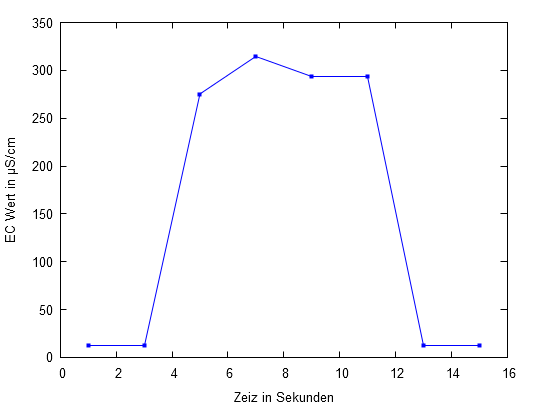
\includegraphics[height=3.0in]{ec_tests}}
\end{minipage}
\vskip0.5cm
Wie erwartet, steigt der EC Wert beim Eintauchen ins Wasser, da es nat\"urlich um einiges leitf\"ahiger ist, als Luft.

\subsection{PH Wert}
\paragraph{Allgemein} \mbox{} \\
Der PH Wert ist einer der wichtigsten Werte, wenn es um das \"Uberwachen eines Aquaponik Systems geht. Daf\"ur gibt es ein gro{\ss}es Spektrum an erh\"altlichen Sensoren. Die der unteren Preisklasse, ben\"otigen eine regelm\"a{\ss}ige Wartung. Die der oberen Preisklasse heben den Preis des Produktes, \"uber die Zielgruppe hinaus, und sind deshalb unmbrauchbar. \\
Da der Sensor ein analoges Signal liefert, muss die gemessene Spannung erst umgerechnet werden. Dies \"ubernimmt die Klasse OpenAquarium.

\begin{lstlisting} [frame=single]
OpenAquarium.calibratepH(cp4,cp7,cp10);
int mvpH = OpenAquarium.readpH(); //Value in mV of pH
float pH = OpenAquarium.pHConversion(mvpH);
\end{lstlisting}
cp4, cp7, cp7 ... Calibrationpoints (Konstanten)

\paragraph{Calibrationpoints} \mbox{} \\
Calibrationpoints (Kalibrierungswerte), werden angepasst, wenn der gemessene PH Wert zu stark vom eigentlichen Wert abweicht. Um die Abweichung des Sensors zu beheben, sind Kalibrierungskits vorgesehen, die allerdings bis zu ein mal im Monat verwendet werden m\"ussen. Dies belastet den Kunden mit zus\"atzlichen Kosten und Aufwand und soll daher umgangen werden.
\paragraph{Tests} \mbox{} \\
Beim testen eines bereits l\"anger in Betrieb gewesenem PH Sensor brachte dieser folgende Ergebnisse: \\
\begin{minipage}{5in}
  \centering
  \raisebox{-0.5\height}{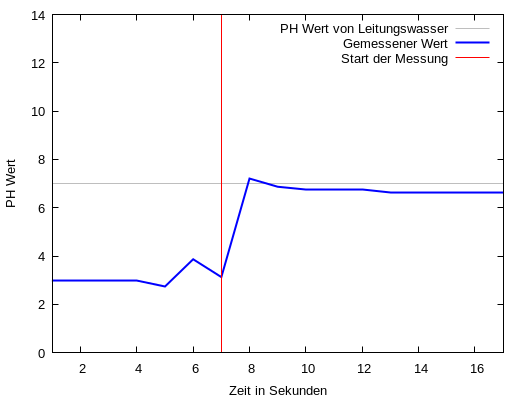
\includegraphics[height=3.0in]{ph_tests}}
\end{minipage}
Wie zusehen ist, weicht der gemessene Wert bereits stark von dem eigentlichen Wert ab. In einem Aquaponik System hat eine Abweichung dieser gr\"o{\ss}e, starke Auswirkungen auf das Gleichgewicht des Ecosystems. \\
\paragraph{Fazit} \mbox{} \\
Da es keine PH Sensoren gibt, die billig sind und zugleich einen niedrigen Warungsaufwand aufweisen, wird je nach M\"oglichkeiten versucht eine eigene L\"osung zu etablieren. Dies soll mithilfe einiger Teststreifen und einer Kamera passieren, bei der, der Benutzer per Knopfdruck \"uber die Website den PH Wert messen kann. Die Vorteile bei dieser L\"osung sind, dass solch ein System einzigartig auf dem Markt w\"are, und dass der Benutzer selbst bestimmen kann, ob er den PH Wert messen will und wie oft. Wie genau dieses System realisiert wird, wird im n\"achsten Sprint (Sprint 1) geplant.
\subsection{Abnahme}
\begin{table}[ht]
  \centering
  \begin{tabular}{lllll}
    \cline{1-3}
    \multicolumn{3}{|c|}{\textbf{\rule{0pt}{4ex}Abnahme User Story 1975 - Sensoren}}
    & \textbf{} &  \\ \cline{1-3}
    \multicolumn{1}{|c|}{\textbf{\rule{0pt}{3ex}Rolle}}     & \multicolumn{1}{c|}{\textbf{Name}} & \multicolumn{1}{c|}{\textbf{Unterschrift}} & \textbf{} &  \\ \cline{1-3}
    \multicolumn{1}{|l|}{\rule{0pt}{3.5ex}Autor}              & \multicolumn{1}{l|}{M. Schwebler}    & \multicolumn{1}{l|}{}                      &           &  \\ \cline{1-3}
    \multicolumn{1}{|l|}{\rule{0pt}{3.5ex}Qualit\"atssicherung} & \multicolumn{1}{l|}{R. Bahadoorifar}       & \multicolumn{1}{l|}{}                      &           &  \\ \cline{1-3}
    \multicolumn{1}{|l|}{\rule{0pt}{3.5ex}Product Owner}      & \multicolumn{1}{l|}{S. Schober}    & \multicolumn{1}{l|}{}                      &           &  \\ \cline{1-3}
    &                                    &                                            &           &  \\
    &                                    &                                            &           &  \\
    &                                    &                                            &           &  \\
    &                                    &                                            &           &
  \end{tabular}
\end{table}
\newpage
\newpage
\section{Aktoren}
Es werden insgesamt vier Aktoren von Ponix Systems zur Verf\"ugung gestellt. Darunter befinden sich: 2 Pumpen (Wasser/Mineralien), 1 Futterautomat und eine Pflanzenbeleuchtung. \\
Um dem Kunden die Arbeit abzunehmen die Zimmertemperatur so zu regulieren um ein Klima f\"ur die Fische zu schaffen, wird zus\"atzlich ein Hitzestrahler verbaut. Dieser wird im n\"achsten Sprint (Sprint 1) geplant und eingesetzt.
\subsection{Pumpe}
\paragraph{Wasser} \mbox{} \\
Die Wasserpumpe kann mit einer Zeile Code ein bzw. ausgeschalten werden. Die Steuerung, die kontrolliert wann genau die Pumpe eingeschalten wird, muss erst implementiert werden (Sprint 1).

\begin{lstlisting} [frame=single]
OpenAquarium.pumpON(1); 
OpenAquarium.pumpOFF(1);
\end{lstlisting}
Zum Anschlie{\ss}en der Pumpe sind auf dem AquariumBoard Steckplätze vorgesehen. \\
\begin{minipage}{5in}
  \centering
  \raisebox{-0.5\height}{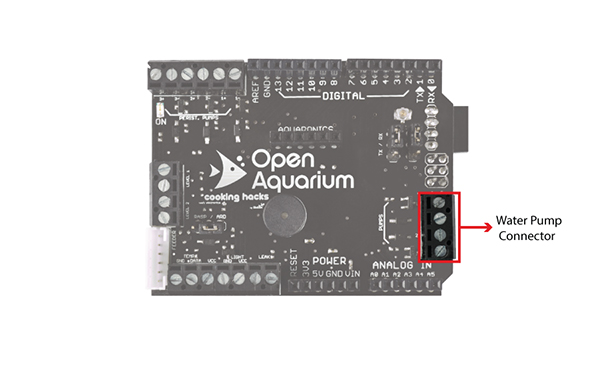
\includegraphics[height=2.3in]{water_pump_connection}}
\end{minipage}
Pumpleistung: 100-350 L/H \\
Spannung: 3.5-12 DC \\
Leistungsbereich: 0.5W-5W \\
\newpage

\paragraph{Mineralien}\mbox{} \\
Wie bei der Wasserpumpe ist der Code zum Aktivieren und Deaktivieren der Pumpe kurz.
\begin{lstlisting} [frame=single]
OpenAquarium.perpumpON(1); 
OpenAquarium.perpumpOFF(1);
\end{lstlisting}
Die Dosierung der Mineralien muss nicht manuell vorgenommen werden sondern kann über das OpenAquarium.h File angepasst werden.
\begin{lstlisting} [frame=single]
#define dosingdrop1 5
#define dosingdrop1 10
#define dosingdrop1 15
\end{lstlisting}
Zum Anschließen der Pumpe sind wieder Steckplätze vorhanden. \\
\begin{minipage}{5in}
  \centering
  \raisebox{-0.5\height}{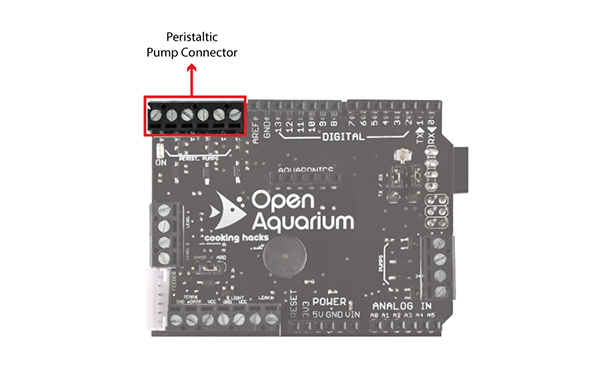
\includegraphics[height=2.3in]{mineral_pump_connection}}
\end{minipage} 
12V DC input voltage \\
Flow: 20-60 ml/min
\newpage

\subsection{Futterautomat}
Um den Wartungsaufwand zu minimieren, ist ein Futterautomat notwendig, der \"uber eine Weboberfl\"ache konfiguriert werden kann. Es kann entweder ein teurer Futterautomat gekauft werden, der diese Option anbietet, oder ein durchschnittlicher Futterautomat wird so bearbeitet, dass er auf ein Stromsignal reagiert indem er Futter ausgibt. \\
Der Futterautomat von Ponix Systems geh\"ort zur letzteren Art. Sobald 5 Volt angelegt wird, gibt er Futter aus. So kann sp\"ater \"uber die WebApp das Intervall und die Menge gesteuert werden.
\subsection{Pflanzenbeleuchtung}
Die Beleuchtung wird mit einem LED Streifen realisiert von www.cooking-hacks.com (bzw. von Ponix Systems gesponsort) realisiert. Er besteht aus 72 LEDs (60 Weiße und 12 Blaue) mit einer Leuchtkraft von 500 Lumen. Der Streifen kann mit Hilfe der OpenAquarium Klasse der aktuellen Zeit automatisch angepasst werden.
\begin{lstlisting} [frame=single]
now = OpenAquarium.getTime();
OpenAquarium.printTime(now);
OpenAquarium.lighting(now);
\end{lstlisting}
Wie bei den beiden Pumpen kann der LED Streifen am OpenAquarium Board angeschlossen werden. \\
\begin{minipage}{5in}
  \centering
  \raisebox{-0.5\height}{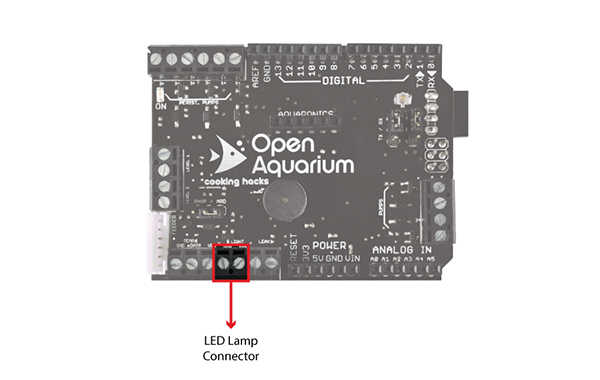
\includegraphics[height=2.2in]{led_connection}}
\end{minipage} 
Leistung: 5.5 watts \\
Beleuchtung: 72 LEDs \\
Farbe: 60 Weiße + 12 Blaue) \\



\subsection{Abnahme}
\begin{table}[ht]
  \centering
  \begin{tabular}{lllll}
    \cline{1-3}
    \multicolumn{3}{|c|}{\textbf{\rule{0pt}{4ex}Abnahme User Story 1979 - Aktoren}}
    & \textbf{} &  \\ \cline{1-3}
    \multicolumn{1}{|c|}{\textbf{\rule{0pt}{3ex}Rolle}}     & \multicolumn{1}{c|}{\textbf{Name}} & \multicolumn{1}{c|}{\textbf{Unterschrift}} & \textbf{} &  \\ \cline{1-3}
    \multicolumn{1}{|l|}{\rule{0pt}{3.5ex}Autor}              & \multicolumn{1}{l|}{Matthias Schwebler}    & \multicolumn{1}{l|}{}                      &           &  \\ \cline{1-3}
    \multicolumn{1}{|l|}{\rule{0pt}{3.5ex}Qualit\"atssicherung} & \multicolumn{1}{l|}{Konrad Kelc}       & \multicolumn{1}{l|}{}                      &           &  \\ \cline{1-3}
    \multicolumn{1}{|l|}{\rule{0pt}{3.5ex}Product Owner}      & \multicolumn{1}{l|}{Samuel Schober}    & \multicolumn{1}{l|}{}                      &           &  \\ \cline{1-3}
    &                                    &                                            &           &  \\
    &                                    &                                            &           &  \\
    &                                    &                                            &           &  \\
    &                                    &                                            &           &
  \end{tabular}
\end{table}

\newpage
\section{Datenbankmanagementsystem}

\subsection{Evaluierung RDBMS vs. NoSQL}

\subsubsection{Einleitung}
Zur Speicherung der Sensordaten soll ein geeignetes Datenbankmanagement-\\ system verwendet werden. Zu Beginn wird evaluiert, ob ein relationales oder ein NoSQL-Datenbanksystem verwendet wird. Dabei werden die jeweiligen Vor-und Nachteile von SQL und NoSQL Datenbanken aufgelistet. Besonders wert gelegt wird auf die Performance, die Konsistenz sowie dem einfachen Zugriff auf die Daten.

\subsubsection{Kriterien}

\begin{itemize}
	\item Performance: \\Gibt an, wie schnell die Lese- und Schreibleistung ist.
	\item Konsistenz: \\Gibt an, wie gut das DBMS Ma{\ss}nahmen zur Konsistenzerhaltung umsetzt.
	\item einfacher Zugriff auf Daten: \\Gibt an, wie Umfangreich die API des DBMS ist.
\end{itemize}

\subsubsection{Optionen}

\paragraph{SQl-Datenbanken}

\textbf{Abfragesprache}\\\\
Die Abfragesprache SQL wir auf die drei Teile DDL(Data Definition Language),
DML(Data Manipulation Language) und DCL (Data Control Language) aufgeteilt.

\begin{itemize}
	\item DDL:\\ ist die Sprache f\"ur das Anlegen, \"Andern und L\"oschen von Datenstrukturen.
	\item DML:\\ ist die Sprache f\"ur das Abfragen, Einf\"ugen, \"Andern oder L\"oschen von Nutzdaten.
	\item DCL:\\ ist die Sprache f\"ur die Zugriffskontrolle.
\end{itemize}
\textbf{Konsistenz}\\\\
SQL-Datenbanken verwenden das ACID Prinzip, daher besitzen sie eine bessere Konsistenz als
NoSQL-Datenbanken. NoSQL Datenbanken verwenden das BASE Prinzip, die Daten hier sind daher
nur "schlussendlich" konsistent. Dadurch kann es passieren das nach einem Update nicht immer
die selben Werte zur\"uckgeliefert werden.

\paragraph{NoSQl-Datenbanken}
NoSQL-Datenbanken besitzen wegen ihres einfachen Schemas eine hohe Skalierbarkeit, welche trotz eines
hohen Datenvolumens gew\"ahrt wird.

\subsubsection{Fazit}
SQL-Datenbanken weisen eine bessere Konsistenz auf, jedoch besitzen NoSQL-Datenbanken
eine bessere Performance und Skalierbarkeit. Da wir besonderen Wert auf die Performance
legen, haben wir uns entschieden eine NoSQL-Datenbank zu verwenden.

\subsection{Evaluierung eines NoSQL Datenbanksystems}

\subsubsection{Einleitung}
Die Folgenden Datebankmanagementsysteme wurden evaluiert:

\begin{itemize}
	\item MongoDB
	\item Redis
\end{itemize}

\subsubsection{Kriterien}

\begin{itemize}
	\item Performance: \\Gibt an, wie schnell die Lese- und Schreibleistung ist.
	\item einfacher Zugriff auf Daten: \\Gibt an, wie Umfangreich die API des DBMS ist.
	\item Dokumentation:\\ Gibt an, wie gut das DBMS dokumentiert ist.
	\item Verbreitung:\\ Gibt an, wie weit das DBMS verbreitet ist.
\end{itemize}

\subsubsection{Optionen}

\paragraph{MongoDB}
MongoDB ist eine Schema-freie, dokumentenorientierte NoSQL-Datenbank, die in der Programmiersprache C++ geschrieben ist. Da die Datenbank dokumentenorientiert ist, kann sie Sammlungen von JSON-\"ahnlichen Dokumenten verwalten. So k\"onnen viele Anwendungen Daten auf nat\"urlichere Weise modellieren, da die Daten zwar in komplexen Hierarchien verschachtelt werden k\"onnen, dabei aber immer abfragbar und indizierbar bleiben.\\\\
Au{\ss}erdem ist MongoDB eine Allzweckdatenbank mit offenem Quellcode (OpenSource).
Sie hat u.a. folgende Merkmale:

\begin{itemize}
	\item Dokumentdatenmodell mit dynamischen Schemata
	\item Umfassende, flexible Indexunterst\"utzung
	\item Aggregation-Framework und MapReduce
	\item Auto-Sharding f\"ur horizontale Skalierbarkeit
	\item Eingebaute Replikation f\"ur Hochverf\"ugbarkeit
	\item Textsuche
	\item Erweiterte Sicherheit (z.B. Kerberos Unterst\"utzung)
	\item Speicherung gro{\ss}er Dateien mit GridFS
\end{itemize}

\paragraph{Redis}
Redis ist eine In-Memory-Datenbank mit einer einfachen Schl\"ussel-Werte-Datenstruktur. Nach einer Erhebung von DB-Engines.com ist Redis der verbreitetste Schl\"ussel-Werte-Speicher.\\
Die einfache Struktur der Datenbank eignet sich weniger f\"ur komplexe Datenstrukturen, die \"uberwiegend in der Datenbank selbst abgebildet werden soll, daf\"ur ist der gro{\ss}e Vorteil von Redis, dass es schneller ist als relationale Datenbanken wie z.B. MySQL. Bis zu ca. 100.000 Schreibvorg\"ange und ca. 80.000 Lesevorg\"ange pro Sekunde sind auf herk\"ommlicher Hardware m\"oglich.\\
Redis bietet Persistenz durch automatisiertes regelm\"a{\ss}iges Abspeichern oder per Protokolldatei, wodurch bei entsprechender Konfiguration auch eine ACID-konforme Dauerhaftigkeit erreichbar ist.

\subsubsection{Fazit}
Redis schneidet bei den Kriterien, wie z.B. der Performance und den einfachen Zugriff auf Daten durch
seine Kompaktheit, besser als MongoDB ab, hat jedoch den gro{\ss}en Nachteil, dass es bei serverseitiger Verwendung, extrem viel Arbeitsspeicher verbraucht, wenn einige Aquaponik Systeme ihre Daten \"uber den Server persistieren.

\subsection{Gesamtfazit}
Es m\"ussen sowohl auf dem lokalen Raspberry Pi, als auch auf dem Server Echtzeitdaten vorhanden sein, um einerseits auf dem Touchdisplay eine \"Ubersicht anzuzeigen und andererseits \"uber den Browser alle Daten zu betrachten. Da auf dem Raspberry Pi allerdings nicht viel Speicherplatz aber gen\"ugend Arbeitsspeicher vorhanden ist, wird daf\"ur Redis verwendet und f\"ur die serverseitige Persistierung MongoDB.

\begin{table}[ht]
  \centering
  \begin{tabular}{lllll}
    \cline{1-3}
    \multicolumn{3}{|c|}{\textbf{\rule{0pt}{4ex}Abnahme User Story 1819 - Datenbankmanagementsystem}}
    & \textbf{} &  \\ \cline{1-3}
    \multicolumn{1}{|c|}{\textbf{\rule{0pt}{3ex}Rolle}}     & \multicolumn{1}{c|}{\textbf{Name}} & \multicolumn{1}{c|}{\textbf{Unterschrift}} & \textbf{} &  \\ \cline{1-3}
    \multicolumn{1}{|l|}{\rule{0pt}{3.5ex}Autor}              & \multicolumn{1}{l|}{Konrad Kelc}    & \multicolumn{1}{l|}{}                      &           &  \\ \cline{1-3}
    \multicolumn{1}{|l|}{\rule{0pt}{3.5ex}Qualit\"atssicherung} & \multicolumn{1}{l|}{Matthias Schwebler}       & \multicolumn{1}{l|}{}                      &           &  \\ \cline{1-3}
    \multicolumn{1}{|l|}{\rule{0pt}{3.5ex}Product Owner}      & \multicolumn{1}{l|}{Samuel Schober}    & \multicolumn{1}{l|}{}                      &           &  \\ \cline{1-3}
    &                                    &                                            &           &  \\
    &                                    &                                            &           &  \\
    &                                    &                                            &           &  \\
    &                                    &                                            &           &
  \end{tabular}
\end{table}
\newpage

\section{Web Framework}
Bei Web Frameworks, werden durch vordefinierte und vorgefertigte Klassen, h\"aufig gebrauchte Funktionen wie Mailversand, sichere Authentifizierung, Sicherheitsfunktionen, Lokalisierung, Performance (z.B. HTTP Caching) oder grundlegende Funktionen f\"ur Webformulare vereinfacht. \\
Web Frameworks sind darauf ausgelegt, sehr schnell Ergebnisse zu erzielen und lauff\"ahige Webanwendungen zu erstellen. Dazu bieten sie einen Datenbankzugriff, Templating-Mechanismen, eine saubere Trennung von Pr\"asen-tation und Code durch Verwendung des Model-View-Controllers. \\
Da eine eigenst\"andige Implementierung all dieser Mechanismen den Arbeitsaufwand \"ubersteigen w\"urde, ist eine Verwendung eines solchen Web Frameworks unabdinglich. Welches Framework dabei gew\"ahlt wird h\"angt von folgenden Komponenten ab:
\begin{itemize}
\item Schwierigkeitsgrad
\item Lernkurve
\item Sicherheit
\item Dokumentation
\end{itemize}
\newpage
\subsection{Django}
Django ist ein in Python geschriebenes opensource Web Application Framework, das einem Model-View-Presenter-Schema folgt.
\paragraph{Schwierigkeitsgrad/Lernkurve} \mbox{}\\
Da Python selbst leicht zu erlernen ist, ist es keine Herausforderung sich in die Sprache einzuarbeiten. Das Framework ansich, gilt als eines der einfachereren (aber auch funktionsarmeren) seiner Art und bietet daher eine flache Lernkurve. F\"ur jemanden der bereits mit Webframeworks gearbeitet hat, ist Django schnell zu erlernen.
\paragraph{Sicherheit} \mbox{}\\
Django ist so konzipiert, dass die standartm\"a{\ss}ig implementierten Sicherheitsma{\ss}nahmen, f\"ur den gr\"o{\ss}ten Teil der Webentwicklung ausreicht. Da zwischen dem Raspberry Pi und dem Server wenig sicherheitsrelevante Daten ausgetauscht werden, gen\"ugt die Sicherheit von Django.
\paragraph{Dokumentation} \mbox{}\\
Die Dokumentation von Django ist gerade f\"ur Einsteiger optimal, da sie einige n\"utzliche Tutorials bietet. Aber auch f\"ur erfahrene Entwickler ist die Dokumentation gro{\ss}artig.
\newpage

\subsection{Node.js}
Node.js ist eine Event-basierte Plattform, welche nicht blockierend ist. Das bedeutet, dass der Server nicht wartet bis ein Ereignis vollendet wurde, um mit den n\"achsten Aufgaben fortfahren zu k\"onnen. Stattdessen werden Callbacks verwendet, welche dann erst aufgerufen werden, wenn ein bestimmtes Ereignis fertig ausgef\"uhrt wurde, bei dem von einer l\"angeren Dauer ausgegangen wird. W\"ahrenddessen kann der Server andere Aufgaben bearbeiten.

An sich l\"auft Node.js nicht Multi-Threaded, wie man vielleicht erwartet, sondern bearbeitet jede eingehende Verbindung mit einem Thread. Jedoch werden bestimmte Funktionen, wie das Auslesen einer Datenbank oder das Rendern von Templates, intern durch mehrere Threads erledigt, welche dann bei Vollendung den zugewiesenen Callback aufrufen. Durch diese Architektur ist Node.js in vielen Bereichen viel schneller als andere Webserver, die f\"ur jede Verbindung einen Prozess erstellen w\"urden.

Node.js ist sehr abh\"angig durch Third-Party Module, welche durch NPM (Node Package Manager) verwaltet und installiert werden k\"onnen. Diese Module machen das Entwickeln von Applikationen viel einfacher oder geben auch mehr Funktionen. F\"ur uns interessante Module w\"aren zum Beispiel: Express.js oder Socket.io. Ersteres gibt uns die M\"oglichkeit die Applikation im MVC-Pattern zu entwickeln.
Mit Socket.io k\"onnte man Daten dem Client senden und gleichzeitig empfangen, ohne dabei davor eine Anfrage vom Client erwarten zu m\"ussen. Es gen\"ugt damit nur noch eine Anfrage vom Client bei dem eine Verbindung (Socket) zum Server ge\"offnet wird, sodass man Daten bidirektional senden kann.

\paragraph{Schwierigkeitsgrad/Lernkurve} \mbox{}\\
Wie der Name schon verr\"at verwendet Node.js JavaScript als Programmiersprache. Falls man die Sprache schon kann, wie in unserem Fall, ist eine Lernkurve jeweils in den einzeln verwendeten Modulen sichtbar, die sehr unterschiedlich sind. Somit ist der Schwierigkeitsgrad nicht wirklich einsch\"atzbar. Der Schwierigkeitsgrad in den oben genannten Modulen liegt im mittleren Bereich.

\paragraph{Sicherheit} \mbox{}\\
Node.js hat eine relativ gro{\ss}e Community. Das ist insofern wichtig, da Sicherheitsl\"ucken dadurch schneller gefunden und behoben werden k\"onnen. Jedoch unterscheidet sich die Sicherheit auch in diesem Punkt in den einzelnen Modulen. Somit muss beachtet werden, dass der zu verwendende Modul eine hohe Bekanntheit hat.

\paragraph{Dokumentation} \mbox{}\\
Node.js ist an sich sehr gut dokumentiert und bietet durch eine Vielzahl von Tutorials einen einfachen Einstieg. Von den bekannten Modulen, wissen wir, dass die Dokumentation sehr gut ist, wie bei Socket.io oder Express.js. Au{\ss}erdem wird der Einstieg in diesen Modulen mit verschiedenen Tutorials, die im Internet zu finden sind, sehr einfach gemacht.

\subsection{Laravel}
Laravel ist ein PHP-Framework und wird von vielen Entwickler derzeit als eines der besten Frameworks f\"ur PHP bezeichnet.
Laravel bietet viele Funktionen an, wie Routing, Templating, Unit Testing, usw.

Die Architektur von PHP unterscheidet sich von Node.js sehr stark:
\begin{itemize}
    \item Pro Verbindung wird ein neuer Prozess erstellt. Dies hat bei hoher Nutzzahl zur Folge, dass der Arbeitsspeicher des Servers sehr schnell voll werden kann.
    Node.js verwendet nur einen Thread und erstellt, falls erforderlich, mehrere Threads f\"ur eine jeweilige Aufgabe, welche dann bei erfolgreicher Ausf\"uhrung (also Aufrufen des Callbacks) beendet werden. Wird aber ein Fehler hervorgerufen st\"urzt Node.js komplett ab, wogegen bei PHP nur der Prozess abst\"urzt.
    \item Jedesmal, wenn ein PHP-Skript ausgef\"uhrt wird, wird das Skript neu interpretiert. Dies hat den Vorteil, dass bei einer Code\"anderung nicht der Server neugestartet werden muss. Der Nachteil liegt jedoch in der Performance.
    Bei Node.js wird der Code beim Starten kompiliert. Eine Code\"anderung wirkt sich jedoch solange nicht am Server aus bis Node.js neugestartet wurde. Dies dauert deutlich l\"anger als ein PHP-Server. Dagegen ist die Performance in der Laufzeit deutlich schneller als bei PHP.
    \item Der Code in PHP l\"auft, anders als in Node.js, synchron ab. So muss zum Beispiel f\"ur eine Datenbankverbindung solange gewartet werden, bis diese auch erfolgreich erstellt worden ist. Dies w\"urde die Antwortzeit einer Anfrage sehr beeintr\"achtigen.
\end{itemize}

\paragraph{Schwierigkeitsgrad/Lernkurve} \mbox{}\\
Die Skriptsprache PHP ist sehr einfach zu lernen, genauso wie das Framework Laravel. Jedoch haben die Teammitglieder nicht viel Erfahrung mit PHP, sodass etwas Zeit f\"ur das Lernen vergehen w\"urde.

\paragraph{Sicherheit} \mbox{}\\
Die Standart implementationen und Sicherheitsmaßnahmen sind für den größten Teil der Webentwicklung ausreichend und decken die Ansprüche des Projekts vollständig.

\paragraph{Dokumentation} \mbox{}\\
PHP ansich bietet eine hervorragende Dokumentation mit einigen Beispielen, was den Einstieg in die Sprache erleichtert. In die Dokumentation von Laravel muss man allerdings viel Zeit investieren um sich einzulesen. 

\subsection{Fazit}
\paragraph{Django} \mbox{}\\
F\"ur Einsteiger ist Django definitiv empfehlenswert. Die gute Dokumentation erm\"oglicht es jeden Entwickler mit - egal mit welchen Kenntnissen - sich einen guten \"Uberblick, was f\"ur dieses Projekt bereits ausreichend ist.
\paragraph{Node.js} \mbox{}\\
Node.js kann mit seinen Modulen innovative L\"osungen bieten, wie das schon erw\"ahnte Socket.io-Modul. Au{\ss}erdem besitzt Node.js eine sehr gro{\ss}e Community, die st\"andig w\"achst, wie auch der derzeitige Trend zeigt. Gro{\ss}e Unternehmen, wie Netflix oder Paypal, basieren auf Node.js, aufgrund seiner Schnelligkeit und hohen Skalierbarkeit.
\paragraph{Laravel} \mbox{}\\
PHP bzw. Laravel ist f\"ur unsere Anforderungen nicht besonders gut geeignet, da unser Produkt ein schnelles System erfordert, sowie eine hohe Zahl von Verbindungen. Dies w\"urden wir mit PHP nicht erreichen k\"onnen.
\\ \mbox{} \\
Bewertung der Frameworks nach Schulnotensystem (1 - Sehr gut bis Nicht gen\"ugend - 5)
\begin{table}[ht]
\centering
\begin{tabular}{|l|c|c|c|c|l}
\cline{1-5}
\textbf{Framework} & \multicolumn{1}{l|}{\textbf{Schwierigkeit}} & \multicolumn{1}{l|}{\textbf{Sicherheit}} & \multicolumn{1}{l|}{\textbf{Dokumentation}} & \multicolumn{1}{l|}{\textbf{Erfahrung}} & \\ \cline{1-5}
\textbf{Django}    & 2                                         & 3                                      & 2                                         & 2                                     & \\ \cline{1-5}
\textbf{NodeJS}    & 1                                         & 2                                      & 1                                         & 1                                     & \\ \cline{1-5}
\textbf{Laravel}   & 3                                         & 2                                      & 2                                         & 3                                     & \\ \cline{1-5}
\end{tabular}
\end{table}
\newpage
\begin{table}[ht]
  \centering
  \begin{tabular}{lllll}
    \cline{1-3}
    \multicolumn{3}{|c|}{\textbf{\rule{0pt}{4ex}Abnahme User Story 1818 - Webframework}}
    & \textbf{} &  \\ \cline{1-3}
    \multicolumn{1}{|c|}{\textbf{\rule{0pt}{3ex}Rolle}}     & \multicolumn{1}{c|}{\textbf{Name}} & \multicolumn{1}{c|}{\textbf{Unterschrift}} & \textbf{} &  \\ \cline{1-3}
    \multicolumn{1}{|l|}{\rule{0pt}{3.5ex}Autor}              & \multicolumn{1}{l|}{\begin{tabular}[c]{@{}l@{}}Ramin Bahadoorifar,\\ Matthias Schwebler\end{tabular}}    & \multicolumn{1}{l|}{}                      &           &  \\ \cline{1-3}
    \multicolumn{1}{|l|}{\rule{0pt}{3.5ex}Qualit\"atssicherung} & \multicolumn{1}{l|}{Konrad Kelc}       & \multicolumn{1}{l|}{}                      &           &  \\ \cline{1-3}
    \multicolumn{1}{|l|}{\rule{0pt}{3.5ex}Product Owner}      & \multicolumn{1}{l|}{Samuel Schober}    & \multicolumn{1}{l|}{}                      &           &  \\ \cline{1-3}
    &                                    &                                            &           &  \\
    &                                    &                                            &           &  \\
    &                                    &                                            &           &  \\
    &                                    &                                            &           &
  \end{tabular}
\end{table}
\newpage

\section{Art der Daten\"ubermittlung}
Bei der Daten\"ubertragung sind mehrere Parameter zu beachten. Dazu geh\"oren haupts\"achlich das Format der Daten und das Intervall in denen diese \"ubertragen werden.
\subsection{Arduino zu Raspberry Pi und vice versa}
Um die Sensordaten dem Raspberry Pi mitzuteilen, eignet sich am besten ein Key-Value Format. Dabei gibt es verschiedene M\"oglichkeiten, wie z.B. JSON und CSV. \\
Das Intervall der Daten\"ubertragung kann frei, vom Benutzer gew\"ahlt werden.
\subsubsection{JSON}
JSON (JavaScript Object Notation) hat den gro{\ss}en Vorteil, der leichten Server-seitigen Auswertung und Konvertierung in ein Javascript Object. Da die Daten aber vor\"ubergehend auf dem Raspberry Pi persistiert werden sollen, und Redis kein automatisches speichern von JSON Objekten unterst\"utzt erzeugt diese Methode der \"Ubertragung mehr Aufwand als Nutzen.
\subsubsection{CSV}
\"Ahnlich wie bei JSON, m\"ussten die Daten erst bearbeitet und gefiltert werden, um in die Datenbank gespeichert werden zu k\"onnen.
\subsubsection{Eigenes Format}
Um die Daten mit Redis zu persistieren wird folgende Syntax verwendet: "Key1 Value1 Key2 Value2 ...". Um Mehraufwand durch Verwendung eines standartisierten Datenformats zu vermeiden, k\"onnen die Daten gleich so gesendet werden, dass sie ohne Bearbeitung in Redis gespeichert werden k\"onnen.
\subsubsection{Fazit}
Der Datenaustausch wird in folgendem Format stattfinden:
\begin{lstlisting} [frame=single]
	temperature 23.4 ec 285.7
\end{lstlisting}

\subsection{Raspberry Pi zu Server und vice versa}
Wenn die Daten in Redis gespeichert worden sind, m\"ussen diese dem Zentralserver gesendet werden. Der Sender auf dem Raspberry Pi ist Node.js, wie auf dem Empf\"anger bzw. Server.

Die Daten schauen bei Auslesen der Datenbank wie folgt aus:
\begin{lstlisting} [frame=single]
	1) temperature
	2) 23.4
	3) ec
	4) 285.7
\end{lstlisting}

Wie wir in Kapitel 10.1 festgestellt haben, offenbart sich die \"Ubertragung in JSON nicht nur wegen der Einfachheit der Konvertierung zu einem Javascript Objekt als Vorteil, sondern auch aus drei anderen Gr\"unden:
\begin{itemize}
    \item \textbf{Einfache Speicherung in MongoDB:} Da MongoDB JSON als Speicherformat verwendet, ist es deswegen f\"ur uns einfacher JSON-Objekte in die Datenbank zu speichern.
    \item \textbf{\"Ubertragung der Daten durch Socket.io:} Daten werden standardm\"a{\ss}ig in Socket.io als JSON-Objekt gesendet.
    \item \textbf{Oberfl\"ache der Webapplikation durch Angular:} Angular bietet Funktionen an, JSON-Objekte in der Weboberfl\"ache anzeigen zu lassen. Falls sich das JSON-Objekt ver\"andert, wird automatisch auch die Oberfl\"ache dementsprechend angepasst.
\end{itemize}

Deswegen werden die Daten wie folgt ausschauen:
\begin{lstlisting} [frame=single]
	{
	  temperature: "23.4",
	  ec: "285.7"
	}
\end{lstlisting}
\newpage
\subsection{Abnahme}
\begin{table}[ht]
  \centering
  \begin{tabular}{lllll}
    \cline{1-3}
    \multicolumn{3}{|c|}{\textbf{\rule{0pt}{4ex}Abnahme User Story 2049 - Art der Daten\"ubermittlung}}
    & \textbf{} &  \\ \cline{1-3}
    \multicolumn{1}{|c|}{\textbf{\rule{0pt}{3ex}Rolle}}     & \multicolumn{1}{c|}{\textbf{Name}} & \multicolumn{1}{c|}{\textbf{Unterschrift}} & \textbf{} &  \\ \cline{1-3}
    \multicolumn{1}{|l|}{\rule{0pt}{3.5ex}Autor}              & \multicolumn{1}{l|}{\begin{tabular}[c]{@{}l@{}}Matthias Schwebler,\\ Ramin Bahadoorifar\end{tabular}}    & \multicolumn{1}{l|}{}                      &           &  \\ \cline{1-3}
    \multicolumn{1}{|l|}{\rule{0pt}{3.5ex}Qualit\"atssicherung} & \multicolumn{1}{l|}{Konrad Kelc}       & \multicolumn{1}{l|}{}                      &           &  \\ \cline{1-3}
    \multicolumn{1}{|l|}{\rule{0pt}{3.5ex}Product Owner}      & \multicolumn{1}{l|}{Samuel Schober}    & \multicolumn{1}{l|}{}                      &           &  \\ \cline{1-3}
    &                                    &                                            &           &  \\
    &                                    &                                            &           &  \\
    &                                    &                                            &           &  \\
    &                                    &                                            &           &
  \end{tabular}
\end{table}
\newpage
\section{Fazit des kompletten Systems}
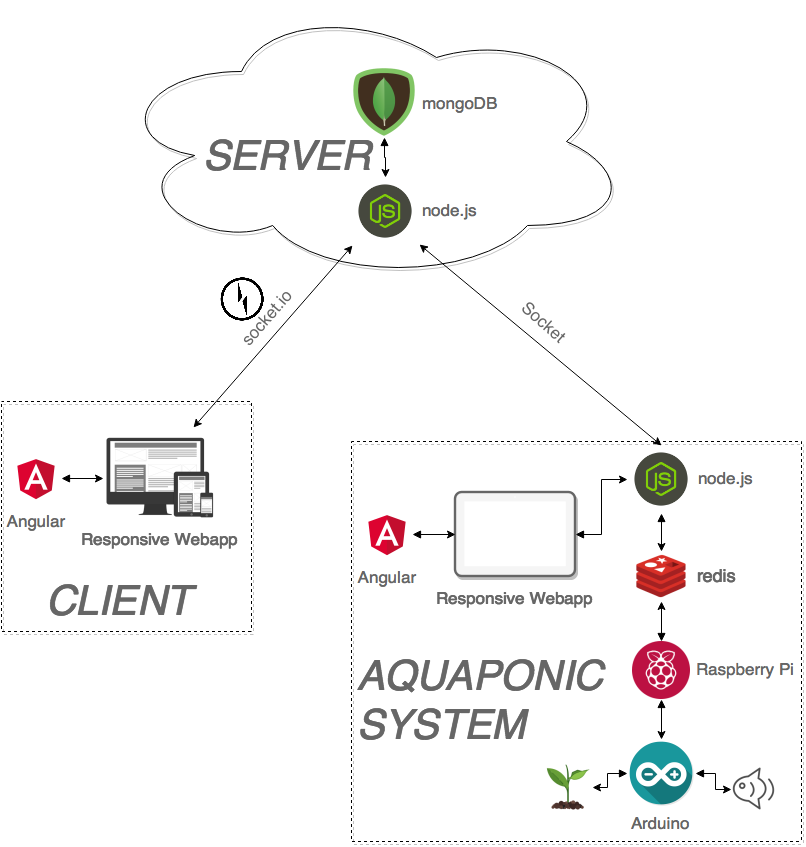
\includegraphics[height=5.3in]{complete_system}
\end{document}
